\section{Model Checking}
Para nuestro sistema de detección de metales pesados, se define un modelo que involucra dos subsistemas independientes que aseguran no estar simultáneamente en estado de alerta.

\subsection*{Variables del Modelo}
\begin{itemize}
    \item \textbf{System1:} Puede estar en los estados \textit{AlertaOn} o \textit{AlertaOff}.
    \item \textbf{System2:} Puede estar en los estados \textit{AlertaOn} o \textit{AlertaOff}.
\end{itemize}

\subsection*{Transiciones del Modelo}
Las transiciones para cada subsistema son las siguientes:
\begin{itemize}
    \item \textbf{System1:}
    \begin{itemize}
        \item Desde \textit{AlertaOff}, puede ir a \textit{AlertaOn} o permanecer en \textit{AlertaOff}.
        \item Desde \textit{AlertaOn}, solo puede ir a \textit{AlertaOff}.
    \end{itemize}
    \item \textbf{System2:}
    \begin{itemize}
        \item Desde \textit{AlertaOff}, puede ir a \textit{AlertaOn} o permanecer en \textit{AlertaOff}.
        \item Desde \textit{AlertaOn}, solo puede ir a \textit{AlertaOff}.
    \end{itemize}
\end{itemize}

\subsection*{Especificaciones del Modelo}
Las siguientes especificaciones aseguran el comportamiento correcto de los subsistemas:
\begin{itemize}
    \item \textbf{CTL:}
    \begin{itemize}
        \item $AG \neg(System1 = AlertaOn \land System2 = AlertaOn)$: Siempre es cierto que ambos sistemas no están en estado \textit{AlertaOn} simultáneamente.
        \item $EF\ System1 = AlertaOn$: Eventualmente, el sistema 1 llega al estado \textit{AlertaOn}.
        \item $EF\ System2 = AlertaOn$: Eventualmente, el sistema 2 llega al estado \textit{AlertaOn}.
        \item $AG\ (System1 = AlertaOff \rightarrow AX\ System1 = AlertaOn)$: Si \textit{System1} está en \textit{AlertaOff}, en el siguiente estado puede ir a \textit{AlertaOn}.
    \end{itemize}
    \item \textbf{LTL:}
    \begin{itemize}
        \item $F\ (System1 = AlertaOn)$: En algún momento, \textit{System1} estará en \textit{AlertaOn}.
        \item $G\ (System1 = AlertaOn \rightarrow X\ System1 = AlertaOff)$: Siempre que \textit{System1} esté en \textit{AlertaOn}, cambiará a \textit{AlertaOff} en el siguiente estado.
    \end{itemize}
\end{itemize}

\subsection*{Descripción del Modelo}
El modelo simula dos sistemas que operan independientemente con transiciones entre estados \textit{AlertaOn} y \textit{AlertaOff}. Garantiza que ambos sistemas no estén en estado de alerta simultáneamente.

\begin{lstlisting}
MODULE main
VAR
  System1 : {AlertaOn, AlertaOff};
  System2 : {AlertaOn, AlertaOff};

ASSIGN
  init(System1) := AlertaOff;
  init(System2) := AlertaOff;

  next(System1) := case
    System1 = AlertaOff : {AlertaOn, AlertaOff};
    System1 = AlertaOn : {AlertaOff};
    TRUE : System1;
  esac;

  next(System2) := case
    System2 = AlertaOff : {AlertaOn, AlertaOff};
    System2 = AlertaOn : {AlertaOff};
    TRUE : System2;
  esac;

SPEC AG !(System1 = AlertaOn & System2 = AlertaOn);
SPEC EF System1 = AlertaOn;
SPEC EF System2 = AlertaOn;
SPEC AG (System1 = AlertaOff -> AX System1 = AlertaOn);

LTLSPEC F (System1 = AlertaOn);
LTLSPEC G (System1 = AlertaOn -> X System1 = AlertaOff);
\end{lstlisting}

\begin{figure}
    \centering
    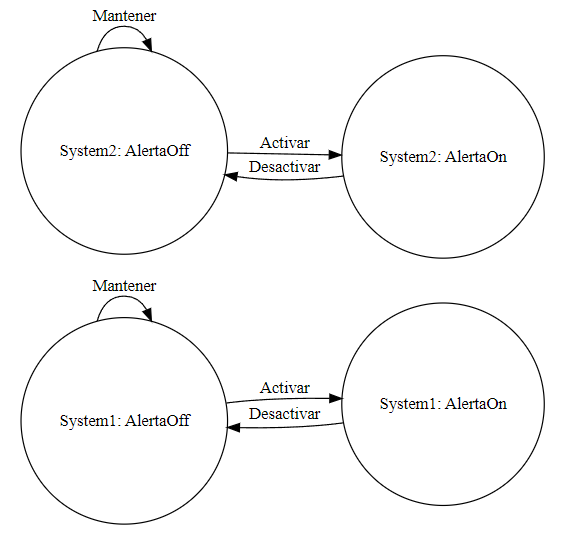
\includegraphics[width=1\linewidth]{Recursos/modelo1.png}
    \caption{Primer Diagrama de Transiciones}
    \label{fig:enter-label}
\end{figure}
